\epigraph{Die Natur faltet, um zu verdichten --- vom Gehirn bis zum Universum.}{}

\section{Die Verformung}


\begin{figure}[ht]
\centering
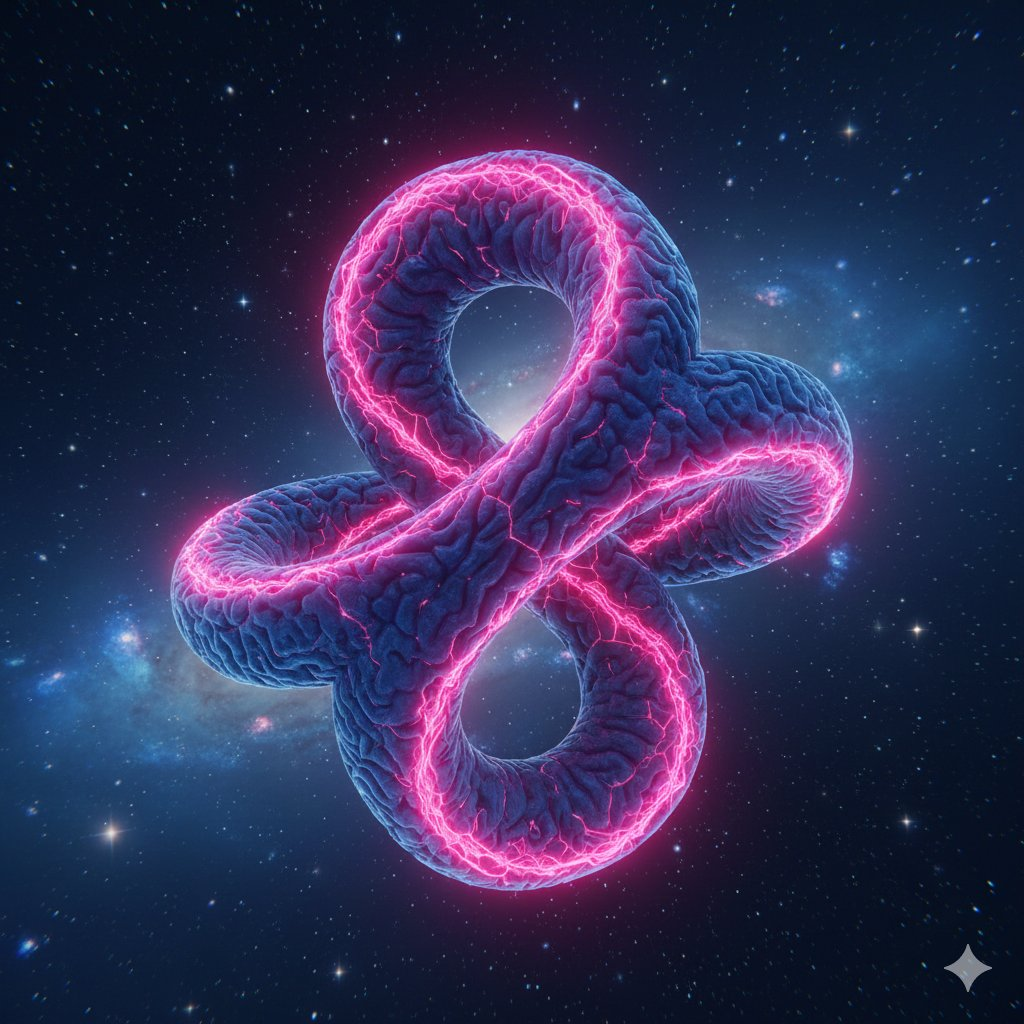
\includegraphics[width=0.75\textwidth]{img/brain_torus_artistic.png}
\caption{Künstlerische Darstellung eines gehirnähnlichen Torus: Ein gefalteter Schlauch mit Gyri-artiger Oberflächenstruktur, durchzogen von Energieflusslinien. Die Vorstellung ist analog zur DNA: So wie sich die Doppelhelix über Nukleosomen, Solenoid-Schleifen und Chromatinfasern zum kompakten Chromosom verklumpt, könnte man sich den Hirnwindungs-Torus als eine ähnliche hierarchische Verdichtung vorstellen --- ein langer, dünner Energieschlauch, der sich auf immer engeren Skalen zusammenfaltet, bis die gefurchte, gehirnähnliche Oberfläche entsteht. \emph{Hinweis:} Dies ist eine stark vereinfachte, künstlerische Visualisierung --- die Abbildung dient der Veranschaulichung des Prinzips, nicht der anatomischen Genauigkeit.}
\label{fig:brain_torus}
\end{figure}
Der ideale, glatte Torus ist ein Ausgangspunkt, aber nicht das Ende der Geschichte. In der physikalischen Realität verformt sich der Torus zu einem \textbf{Hirnwindungs-Torus} --- einer Topologie, die an die Gyri und Sulci der Großhirnrinde erinnert.

Die Analogie ist nicht zufällig. Das menschliche Gehirn löst ein fundamentales geometrisches Problem: Wie maximiert man die Oberfläche (und damit die Verarbeitungskapazität) in einem begrenzten Volumen? Die Antwort der biologischen Entwicklung: durch Faltung. Die Großhirnrinde faltet sich zu Windungen (Gyri) und Furchen (Sulci), wodurch die Oberfläche um ein Vielfaches vergrößert wird. Dass die Natur auf der fundamentalsten und auf der komplexesten Ebene dieselbe geometrische Lösung findet, ist in der T0-Perspektive kein Zufall --- es ist geometrische Notwendigkeit (siehe Kapitel~16).

Dieselbe Lösung wählt die Natur auf der fundamentalsten Ebene. Der vierdimensionale Torsionskristall faltet sich zu einem Windungsgeflecht, in dem die \emph{Wechselwirkungsfläche} dramatisch vergrößert wird --- während das Volumen endlich bleibt.

\section{Teilchen als Resonanzen}

In diesem Bild sind Elementarteilchen keine punktförmigen Objekte und keine Anregungen eines abstrakten Quantenfeldes. Sie sind \textbf{stehende Wellen} --- Resonanzen im Windungsgeflecht des Torus. Ein Elektron ist eine bestimmte Resonanzmode, ein Myon eine andere, ein Tau eine dritte. Die drei Generationen der Teilchenphysik entsprechen drei verschiedenen Resonanzmoden desselben geometrischen Objekts.

Die Kräfte zwischen Teilchen sind \textbf{geometrische Kopplungen} zwischen verschiedenen Torsionsmoden. Elektromagnetismus, schwache und starke Kraft --- sie alle beschreiben, wie verschiedene Resonanzen im Windungsgeflecht miteinander wechselwirken. Und die Massen der Teilchen sind die \textbf{Frequenzen} dieser Resonanzen.

\section{Die Windungszahl und $\xsi$}

Die Windungsdichte bestimmt direkt den Parameter~$\xsi$: Mit $30000/4 = 7500$ Windungen ergibt sich $\xsi = 4/30000$. Das ist die Brücke zwischen der abstrakten Geometrie und dem messbaren Parameter.

\section{Was der Hirnwindungs-Torus erklärt}

Die gefaltete Torusstruktur liefert Erklärungen für drei zentrale Rätsel:

Erstens: \emph{Warum gibt es genau drei Generationen?} Elektron, Myon und Tau sind nicht willkürliche Kopien desselben Teilchens. Sie sind die drei niedrigsten Resonanzmoden des Windungsgeflechts --- vergleichbar mit dem Grundton und den ersten beiden Obertönen einer Saite.

Zweitens: \emph{Warum das Hierarchieproblem?} Die enorme Differenz zwischen der Planck-Energie und der elektroschwachen Skala hat eine geometrische Ursache: Die Planck-Energie verteilt sich über $f^4$ Zellen im vierdimensionalen Hyperwürfel der Torusstruktur. $7500^4 \approx 3{,}16 \times 10^{15}$ --- das ist genau die Größenordnung des Hierarchieproblems.

Drittens: \emph{Warum die Gravitationskonstante so klein ist.} $G$ skaliert mit~$\xsi^2$, und $\xsi$ ist die inverse Windungszahl. Mehr Windungen bedeuten feinere Torsion, und feinere Torsion bedeutet schwächere effektive Gravitation.

\section{Die Zeit im Torus}

Hier liegt vielleicht das konzeptionell Schwierigste: Der Torus kodiert die \emph{Zeit mit}.

In der Standardphysik denkt man in drei Raumdimensionen plus einer separaten Zeitdimension. In T0 ist die Zeit keine externe Koordinate. Sie ist \emph{in der Torusstruktur eingewoben} --- als Phasenentwicklung~$\theta(x)$ des Vakuumfeldes.

Die Phase~$\theta$ des Vakuumfeldes~$\Phi = \rho \cdot e^{i\theta}$ \emph{ist} die Zeit: $\dot{\theta} = m = 1/T$. Zeit ist nicht etwas, das \enquote{vergeht} --- sie ist die \emph{Rotationsrate} des Torus.

Die lokale Zeitrate entspricht der lokalen Windungsgeschwindigkeit der Torusphase. Wo mehr Masse vorhanden ist (höheres~$\rho$), dreht die Phase langsamer --- das \emph{ist} Zeitdilatation. Wo weniger Masse ist, dreht die Phase schneller --- das \emph{ist} die schnellere Zeit im Vakuum.

Die Zeit-Masse-Dualität~$T \cdot m = 1$ ist in diesem Bild keine Postulation, sondern \emph{geometrische Notwendigkeit}: Windungsfrequenz mal Trägheit gleich Konstante auf dem Torus.

\begin{kerngedanke}
Der Torus ist schwer vorstellbar, weil wir Zeit als \enquote{Fluss} erleben. Aber physikalisch ist die Zeit eine Phasenkoordinate auf einer geschlossenen Mannigfaltigkeit --- nicht fundamentaler als der Winkel auf einem Kreis.
\end{kerngedanke}
